\subsection{Теорема об интегрируемости непрерывной на отрезке функции}

Рассматривается вопрос о достаточных условиях интегрируемости функции по Риману. Одним из важнейших классов интегрируемых функций являются функции, непрерывные на отрезке. Доказательство данной теоремы опирается на глубокое свойство непрерывных функций — теорему Кантора о равномерной непрерывности.

\begin{theorem}
Если функция $f(x)$ непрерывна на отрезке $[a, b]$, то она интегрируема по Риману на этом отрезке.
\end{theorem}

\begin{tcolorbox}[title=Доказательство, breakable]
Для доказательства воспользуемся критерием интегрируемости Дарбу: функция интегрируема тогда и только тогда, когда предел разности верхней и нижней сумм Дарбу при стремлении диаметра разбиения к нулю равен нулю.

1. Так как функция $f(x)$ непрерывна на отрезке $[a, b]$, то по теореме Кантора она \textbf{равномерно непрерывна} на этом отрезке. Это означает, что:
\[ \forall \eps > 0 \quad \exists \delta > 0 : \forall x', x'' \in [a, b], \quad |x' - x''| < \delta \implies |f(x') - f(x'')| < \frac{\eps}{b-a} \]

2. Возьмем произвольное разбиение $P$ отрезка $[a, b]$ такое, что его диаметр (мелкость) $\lambda(P) < \delta$. 

3. Рассмотрим разность между верхней и нижней суммами Дарбу для данного разбиения:
\[ S(P) - s(P) = \sum_{j=1}^n M_j \Delta x_j - \sum_{j=1}^n m_j \Delta x_j = \sum_{j=1}^n (M_j - m_j) \Delta x_j \]
где $M_j$ и $m_j$ — точные верхняя и нижняя грани (в силу непрерывности — максимум и минимум) функции $f(x)$ на элементарном отрезке $[x_{j-1}, x_j]$.

4. Величина $\omega_j = M_j - m_j$ называется колебанием функции на отрезке. Поскольку длина каждого отрезка $\Delta x_j \le \lambda(P) < \delta$, то в силу равномерной непрерывности для любых двух точек этого отрезка (включая те, в которых достигаются $M_j$ и $m_j$) выполняется неравенство:
\[ \omega_j = M_j - m_j < \frac{\eps}{b-a} \]

5. Оценим теперь всю сумму:
\[ S(P) - s(P) = \sum_{j=1}^n \omega_j \Delta x_j < \sum_{j=1}^n \frac{\eps}{b-a} \Delta x_j = \frac{\eps}{b-a} \sum_{j=1}^n \Delta x_j \]
Так как сумма длин элементарных отрезков равна длине всего отрезка ($\sum \Delta x_j = b - a$), получаем:
\[ S(P) - s(P) < \frac{\eps}{b-a} (b - a) = \eps \]

6. Таким образом, мы показали, что для любого $\eps > 0$ можно подобрать такой диаметр разбиения $\delta$, что разность сумм Дарбу станет меньше $\eps$. Это означает, что:
\[ \lim_{\lambda(P) \to 0} (S(P) - s(P)) = 0 \]
Следовательно, по критерию Дарбу, функция $f(x)$ интегрируема на $[a, b]$.
\end{tcolorbox}

\subsubsection*{Геометрический смысл}
Непрерывность функции гарантирует отсутствие «скачков» и неограниченных колебаний. С геометрической точки зрения это означает, что при достаточно мелком разбиении площадь ступенчатой фигуры, описанной вокруг графика, и площадь вписанной фигуры будут сколь угодно близки к одной и той же величине — площади криволинейной трапеции.

\subsubsection*{Замечание об ограниченности}
Лектор подчеркивает, что из непрерывности на отрезке автоматически следует ограниченность функции (по первой теореме Вейерштрасса). Это важно, так как ограниченность является необходимым условием интегрируемости по Риману. Если бы функция была непрерывна на интервале, но не ограничена (например, $1/x$ на $(0, 1]$), она не была бы интегрируема.

%\begin{center}
%\includegraphics[width=0.6\textwidth]{continuous_integral.png}
% На рисунке должен быть изображен гладкий график непрерывной функции, 
% разбиение на отрезки и заштрихованная область между верхней и нижней 
% ступенчатыми фигурами, которая становится «узкой» при уменьшении шага.
%\end{center}

\begin{tikzpicture}[>=stealth, scale=1.0]
 
% f(x) = sin(x/2)+2, гладкая и непрерывная
\pgfmathdeclarefunction{ff}{1}{%
  \pgfmathparse{sin(deg(#1*0.55))*1.2+2.3}%
}
 
\def\xa{0.8}
\def\xb{7.8}
\def\N{8}
\pgfmathsetmacro{\dx}{(\xb-\xa)/\N}
 
%--- Верхние прямоугольники S(P) ---
\foreach \j in {1,...,8}{
  \pgfmathsetmacro{\xl}{\xa+(\j-1)*\dx}
  \pgfmathsetmacro{\xr}{\xa+\j*\dx}
  \pgfmathsetmacro{\xm}{(\xl+\xr)/2}
  \pgfmathsetmacro{\va}{ff(\xl)}
  \pgfmathsetmacro{\vc}{ff(\xm)}
  \pgfmathsetmacro{\ve}{ff(\xr)}
  \pgfmathsetmacro{\Mj}{max(\va,max(\vc,\ve))}
  \fill[blue!15] (\xl,0) rectangle (\xr,\Mj);
  \draw[blue!50, line width=0.5pt] (\xl,0) rectangle (\xr,\Mj);
}
 
%--- Нижние прямоугольники s(P) ---
\foreach \j in {1,...,8}{
  \pgfmathsetmacro{\xl}{\xa+(\j-1)*\dx}
  \pgfmathsetmacro{\xr}{\xa+\j*\dx}
  \pgfmathsetmacro{\xm}{(\xl+\xr)/2}
  \pgfmathsetmacro{\va}{ff(\xl)}
  \pgfmathsetmacro{\vc}{ff(\xm)}
  \pgfmathsetmacro{\ve}{ff(\xr)}
  \pgfmathsetmacro{\mj}{min(\va,min(\vc,\ve))}
  \fill[orange!20] (\xl,0) rectangle (\xr,\mj);
  \draw[orange!70, line width=0.5pt] (\xl,0) rectangle (\xr,\mj);
}
 
%--- Кривая ---
\draw[blue!70!black, very thick, domain=0.5:8.2, samples=120]
  plot (\x, {sin(deg(\x*0.55))*1.2+2.3});
 
%--- Оси ---
\draw[->,thick] (0,0)--(9.0,0) node[right]{$x$};
\draw[->,thick] (0,-0.3)--(0,4.5) node[above]{$f(x)$};
 
%--- Точки a и b ---
\foreach \xp/\lab in {\xa/{$a$}, \xb/{$b$}}{
  \draw (\xp,0.07)--(\xp,-0.07);
  \node[below,font=\small] at (\xp,0) {\lab};
}
 
%--- Выделение колебания ω_j для одного отрезка ---
\pgfmathsetmacro{\xl}{\xa+4*\dx}
\pgfmathsetmacro{\xr}{\xa+5*\dx}
\pgfmathsetmacro{\xm}{(\xl+\xr)/2}
\pgfmathsetmacro{\va}{ff(\xl)}
\pgfmathsetmacro{\vc}{ff(\xm)}
\pgfmathsetmacro{\ve}{ff(\xr)}
\pgfmathsetmacro{\Mv}{max(\va,max(\vc,\ve))}
\pgfmathsetmacro{\mv}{min(\va,min(\vc,\ve))}
 
% штриховка зазора
\fill[red!18] (\xl,\mv) rectangle (\xr,\Mv);
\draw[red!50,dashed,thin] (\xl,\mv)--(\xr,\mv) (\xl,\Mv)--(\xr,\Mv);
\draw[<->,red!70,very thin] (\xm+0.15,\mv)--(\xm+0.15,\Mv)
  node[midway,right,font=\scriptsize]{$\omega_j<\dfrac{\varepsilon}{b-a}$};
 
%--- Скобка Δx ---
\draw[<->,gray,thin] (\xl,-0.35)--(\xr,-0.35)
  node[midway,below,font=\scriptsize]{$\Delta x_j$};
 
%--- Пояснение ---
\node[right,font=\small,blue!50] at (7.2,4.1){$S(P)$};
\node[right,font=\small,orange!80!black] at (7.2,3.5){$s(P)$};
\node[blue!70!black,font=\itshape,right] at (8.3,2.7){$f(x)$};
 
\node[font=\small] at (4.5,-0.85)
  {$S(P)-s(P)=\displaystyle\sum_j\omega_j\Delta x_j
    <\frac{\varepsilon}{b-a}(b-a)=\varepsilon$};
 
\end{tikzpicture}